% SHARD-ID: LB-16-NUMERICS
% SHARD-TITLE: Numerics -- models, algorithms, tests, and results
% SHARD-SOURCES: numerics/docs/kink-sector-notes.md, numerics/docs/fm-twomagnon-notes.md,
%   numerics/docs/spin1-twomagnon-notes.md, numerics/src/*.jl, numerics/test/*.jl,
%   numerics/scripts/*.jl, numerics/results/*.json, claims/CLAIMS.md (rows N1, N2, Bc),
%   HANDOFF.md (session-7/8 numerics paragraphs), paper/skeleton.md section 6,
%   theory/lanes/blitz-2026-08-29/wave2-repair/SUMMARY.md
% SHARD-CLAIMS: N1, N2, Bc
%
% Figures are produced by labbook/figures/make_figures.py from the committed
% JSON records; rerun that script after any numerics rerun.

\section{Numerics: models, algorithms, tests, and results}\label{sec:numerics}

% Shard-local typesetting aid (permitted by rule 10 of the writing guide):
% this shard is unusually dense in long, unhyphenatable \texttt{} file and
% checker names.  A little extra emergency stretch, confined to this section
% by the surrounding group, keeps them inside the margin without resorting to
% \sloppy for the whole document.
\begingroup
\emergencystretch=3em

\subsection{What the numerics are for}\label{sec:numerics-role}

The numerical work in this campaign plays two roles and only two.

The first is that of an \emph{oracle}. Several of the theorems in
\cref{sec:two-magnon} and \cref{sec:memory-quantization} are built on
structural facts about a specific model --- a two-magnon scattering phase, a
magnon dispersion, the position of a phase boundary --- which the proofs
consume as inputs. Where such an input can be computed exactly, it is
computed, and the computation is kept next to the proof that uses it.

The second is that of a \emph{falsifier}. A conjecture in this campaign
becomes interesting only once someone has written down, in advance, a number
that it forbids. The spin-$s$ battery of \cref{sec:numerics-bc} is the
clearest instance: before any production run, the two competing hypotheses
were recorded (soft phase slope $1/s$ and memory ratio $-1/s$ if the
conjecture survives; $2$ and $-2$ if it does not), together with a decision
band of eight per cent. The runs were then executed once and the verdict
read off. Nothing was retuned afterwards.

Two disciplines are enforced throughout.

\emph{Red--green development.} Every checked quantity has a test that was
written first and observed to fail first. Two of these failures are recorded
in the source notes because they were instructive rather than clerical: the
first ferromagnetic two-magnon estimator, a windowed centroid of the one-body
density, was biased at the ten-per-cent level and returned the \emph{wrong
sign} for the hard-magnon displacement; and the first spin-$s$ contact
calculation symmetrised a wavefunction that is not symmetric, obtaining a
spin-independent scattering length that would have falsified the conjecture
for the wrong reason. In both cases the numerics caught the error before the
algebra was redone, and in neither case was a tolerance moved to make a test
pass. Tolerance constants are fixed in the test headers before the production
runs and are quoted in this section wherever they carry weight.

\emph{Pre-registration and honest verdicts.} A pass criterion that is chosen
after seeing the data is not a criterion. Where the pre-registered band was
missed, or where a diagnostic turned out to measure something other than what
its name suggested, this is reported in \cref{sec:numerics-honesty} rather
than smoothed over.

One boundary is absolute and is repeated here because it governs how every
number below should be read: \textbf{no numerical result in this campaign
promotes a claim.} A survived falsifier leaves a conjecture a conjecture. The
one claim row that rests on numerics alone --- the empirical XXZ memory scan
--- is held at \statusSketch\ precisely because it is evidence and not a
theorem, and the conjecture the spin-$s$ battery failed to kill remains
\statusConjecture. \Cref{sec:triangle-status} states which corners of the
triangle are carried by proof and which by evidence.

\subsection{The codebase}\label{sec:numerics-code}

The numerics live in a single Julia package, \texttt{TriangleMPS}, under
\texttt{numerics/\allowbreak{}}. It splits into two implementation families that share
conventions and estimators but nothing else.

The \emph{exact-sector family} builds a Hamiltonian directly as a sparse
matrix on an explicitly enumerated basis of a conserved sector, and evolves a
state with a Krylov exponential. It uses no tensor-network library at all:
sparse linear algebra, an eigen-solver and a matrix exponential are the whole
toolkit. Every number it produces is exact up to a stated Krylov tolerance and
a stated basis truncation.

The \emph{uniform-MPS family} works in the thermodynamic limit and in windows
cut out of it, and does use a tensor-network library (\texttt{TensorKit} for
the graded tensors, \texttt{MPSKit} for the variational and time-evolution
algorithms). It is the only part of the campaign where the accuracy is
controlled by a bond dimension rather than by a basis size.

\subsubsection{The three models}

Three Hamiltonians carry all of the numerics.

\emph{(i) The easy-axis spin-$\tfrac12$ XXZ ferromagnet with a frozen kink.}
On $N$ sites,
\begin{equation}
  H \;=\; -\sum_{x=1}^{N-1}\Bigl[\tfrac{J_\perp}{2}\bigl(S^+_xS^-_{x+1}
      + S^-_xS^+_{x+1}\bigr) + J_z\,S^z_xS^z_{x+1}\Bigr],
  \qquad \Delta := J_z/J_\perp > 1,
  \label{eq:num-xxz}
\end{equation}
with $J_\perp = 1$ throughout, so that $J_z=\Delta$. Both terms are
ferromagnetic, so the fully polarised states are exact ground states and $z$
is the easy axis. Sites $1$ and $N$ carry \emph{frozen} classical spins: they
contribute their Ising bonds to their neighbours but cannot flip. With
$\sigma_1=\uparrow$, $\sigma_N=\downarrow$ this realises the one-kink boundary
condition, and it makes the total $S^z$ of the $L=N-2$ dynamical sites exactly
conserved by construction rather than merely energetically. The magnon
dispersion in this convention is
\begin{equation}
  \omega(k) = J_z - J_\perp\cos k, \qquad v_g(k) = J_\perp \sin k,
  \label{eq:num-xxz-disp}
\end{equation}
gapped for $\Delta>1$, and it is reproduced by the code against the exact
open-chain eigenvalues $\omega_m = J_z - J_\perp\cos\bigl(\pi m/(L+1)\bigr)$
to $10^{-10}$. The same construction is carried to general site spin $s$ in
the spin-$s$ modules, with $S^z=+s$ frozen on the left end and $-s$ on the
right.

\emph{(ii) The isotropic spin-$S$ Heisenberg ferromagnet on a ring.} With
$n_x := S - S^z_x$ the on-site magnon number,
\begin{equation}
  H_S \;=\; -J\sum_x\bigl(\mathbf{S}_x\cdot\mathbf{S}_{x+1} - S^2\bigr),
  \label{eq:num-fm}
\end{equation}
whose exact two-magnon form is a diagonal part
$2JS\sum_x n_x - J\sum_{\text{bonds}} n_xn_{x+1}$ together with a hop
amplitude $-\tfrac{J}{2}\sqrt{n_a(2S-n_a+1)}\sqrt{(n_b+1)(2S-n_b)}$ from site
$a$ to site $b$. The free hop is $-JS$; the hop that creates or destroys a
doubly occupied site carries $-Jg$ with $g=\sqrt{S(2S-1)}$, which vanishes at
$S=\tfrac12$ (the hard-core case) and is the entire reason the higher spins
behave differently. The one-magnon dispersion is $\omega(k)=2JS(1-\cos k)$.
For $S\geq 1$ the two-magnon basis has $N(N-1)/2 + N$ states, the extra $N$
being the doubly occupied sites --- a genuine second channel, not
bookkeeping.

\emph{(iii) The anisotropic spin-1 $\lambda$--$D$ chain,} the showcase model.
Note the sign: the overall coupling here is $+J$, antiferromagnetic, the
opposite convention to \cref{eq:num-xxz} and \cref{eq:num-fm}.
\begin{equation}
  H \;=\; J\sum_x\Bigl[S^x_xS^x_{x+1} + S^y_xS^y_{x+1} + \Delta\,S^z_xS^z_{x+1}
     + K\bigl(\mathbf{S}_x\cdot\mathbf{S}_{x+1}\bigr)^2\Bigr]
     + D\sum_x\bigl(S^z_x\bigr)^2 ,
  \label{eq:num-lambdaD}
\end{equation}
with $J=1$ and $S^z$ eigenvalues $\{+1,0,-1\}$. At $K=0$ the $(\Delta,D)$
plane already contains the three phases the campaign needs inside a single
Hamiltonian: a N\'eel phase with $\mathbb{Z}_2$ symmetry breaking and genuine
kinks ($\Delta \gtrsim 1.19$ at $D=0$), the Haldane symmetry-protected phase
($\Delta\approx1$, $D\lesssim0.97$), and a trivial large-$D$ phase
($\Delta\approx1$, $D\gtrsim0.97$). The biquadratic coupling $K$ is carried
only so that the exactly solvable AKLT point $(\Delta,D,K)=(1,0,\tfrac13)$
lies inside the same family and can serve as a closed-form calibration; every
physics point of the campaign has $K=0$. The two string unitaries are
$U_\alpha = \exp(i\pi S^\alpha)$ and the two string order parameters are
\begin{equation}
  \mathcal{O}^\alpha \;=\; -\lim_{r\to\infty}
   \Bigl\langle S^\alpha_1 \Bigl(\textstyle\prod_{1<y<1+r} e^{i\pi S^\alpha_y}\Bigr)
   S^\alpha_{1+r}\Bigr\rangle,
  \qquad \alpha \in \{x,z\},
  \label{eq:num-string}
\end{equation}
normalised so that the AKLT value is $+4/9$. Note that $U_x$ does not conserve
$S^z$, so $\mathcal{O}^x$ is unavailable in the charge-graded code path; this
is why the model is carried in two independent tensor backends (an ungraded
one on $\mathbb{C}^3$, and a $U(1)$-graded one that additionally resolves the
entanglement spectrum by total $S^z$), which are cross-checked against each
other.

\subsubsection{Sector construction and the controlled truncation}

The exact-sector modules never diagonalise the full Hilbert space. For the
kink problem the relevant statement, and it is a correction to the naive
picture, is that a single-domain-wall configuration $\uparrow^a\downarrow^{L-a}$
has $n_{\text{down}} = L-a$, so \emph{different kink positions live in
different $S^z$ sectors}. Each $S^z$ sector therefore contains exactly one
sharp kink, rigidly tied to the sector label, and the kink-plus-one-magnon
space is the neighbouring $S^z$ eigenspace restricted to configurations with
one or three domain walls.

Domain-wall counting is a spin-$\tfrac12$ notion, and the spin-$s$ modules
replace it by the invariant \emph{up-variation}
\begin{equation}
  D(n) \;:=\; \sum_x \max\bigl(0,\; n_x - n_{x+1}\bigr),
  \label{eq:num-upvariation}
\end{equation}
the total upward variation of the magnon number including the frozen ends. A
monotone wall of any width has $D=0$; a wall plus one magnon on either side
has $D=1$. At $s=\tfrac12$ this reduces to $D = (\#\text{domain walls}-1)/2$,
so the cut $D\leq 1$ reproduces the spin-$\tfrac12$ three-wall basis
configuration for configuration --- something the test suite checks
explicitly, together with the equality of the two operators' spectra.

The truncation to $D\leq d_{\max}$ is not an exact sector, because the
elementary exchange move changes the wall count by $0$ or $\pm2$. It is,
however, controlled in three separate senses. It is off-resonant: a
configuration with $k$ extra pairs of walls sits roughly $kJ_z$ above the
one-kink energy, one magnon gap away. It is Hermitian: the code builds
$PHP$, so unitarity and energy conservation of the evolution remain exact and
are measured (norm drift below $2\times10^{-12}$ and energy drift below
$10^{-9}$ across every production run). And it is measurable: the discarded
matrix elements and the weight removed by the state-preparation projection are
both reported. The decisive convergence check is a direct basis enlargement.
At $s=1$, $N=46$, $\Delta=6$, going from $d_{\max}=1$ (dimension $7\,128$) to
$d_{\max}=2$ (dimension $1\,021\,680$) moves the memory ratio by
$1.2\times10^{-4}$ --- a factor $143$ in basis size for a change in the fifth
decimal.

One warning is worth restating, because the diagnostic invites
misreading. The reported Frobenius norm of the discarded matrix elements is
extensive and unnormalised; it grows with basis size and cannot be compared to
unity or read as a relative error. In the accepted spin-$\tfrac12$ runs its
ratio to the retained hopping norm is already $0.99$, while those runs agree
with the exact reference to within a few per cent. What bounds the error is
state-level: initial-state leakage, exact conservation, size convergence, the
basis-enlargement comparison above, and the $s=\tfrac12$ control on the same
code path.

\subsubsection{Time evolution}

Sector ground states in the exact-sector family are obtained by dense
symmetric diagonalisation below dimension $400$ and by Lanczos above it, from
a \emph{deterministic} start vector (the sharp-wall basis vector plus a small
reproducible perturbation), so that every run is bit-reproducible from the
parameters recorded in its own output file.

Time evolution there is Krylov, not Trotter and not Runge--Kutta: one
\texttt{KrylovKit} matrix-exponential call per step (\texttt{krylovdim}$\,=40$,
\texttt{tol}$\,=10^{-12}$ or tighter), stepping the interacting run and, where
a reference is needed, the free runs in lockstep. The step size is a fixed
input; there is no adaptive step control, because the tolerance sits on the
Krylov expansion and the resulting conservation is measured afterwards rather
than assumed. The projected Hamiltonian is Hermitian, so the only error is that
tolerance; accumulated over up to some $550$ steps the measured norm drift
stays below $1.8\times10^{-12}$ and the energy drift below $6.1\times10^{-10}$.

The uniform-MPS family uses three different variational algorithms for three
different geometries. Bulk ground states are found by a tangent-space
uniform-MPS optimisation with the Galerkin gradient as the convergence
measure; a stalled search is restarted from the stalled state, and if it still
does not converge it is handed once to a Riemannian gradient descent with a
different descent direction, the result being reported as measured either way.
Convergence means the Galerkin gradient is below tolerance and nothing weaker.
The kink band is obtained from a quasiparticle (tangent-space) excitation
ansatz in the \emph{topological} sector --- left vacuum $\psi_A$, right vacuum
$\psi_B$, the two broken N\'eel vacua --- so that the excitation returned is a
domain wall rather than a magnon. Finite open chains are prepared by two-site
sweeping density-matrix renormalisation. Real-time evolution is two-site
time-dependent variational principle at a fixed truncation rank, inside a
finite window whose infinite environments are frozen.

The frozen-environment window is an honest limitation, not a formality:
nothing leaving the window comes back, so a readout is only meaningful while
the measured edge leakage is small. The transport records carry the leakage
time series, and the analysis is supposed to restrict the readout to samples
below a fixed leakage tolerance. \Cref{sec:numerics-honesty} reports what
happens when that restriction selects nothing.

\subsubsection{Observables and estimators}

Position estimators for a wall are all \emph{windowed}, on a window $W$ of
half-width $h$ centred on the initial wall. This is forced: an unwindowed
first moment of the magnetisation gradient telescopes to the total
magnetisation, which is exactly conserved, so a global centroid would return
$\delta x \equiv 0$ identically. Three estimators are computed, all exact on a
sharp wall, with $m(x) = \langle S^z_x\rangle$:
\begin{align}
  \hat X_1 &= \frac{\sum_{x\in W}\bigl(x+\tfrac12\bigr)\bigl[m(x)-m(x+1)\bigr]}
                   {\sum_{x\in W}\bigl[m(x)-m(x+1)\bigr]}
             && \text{(gradient centroid),}\label{eq:num-X1}\\
  \hat X_2 &= \frac{1}{2s}\sum_{x\in W} m(x) \;+\; \frac{x_a+x_b}{2}
             && \text{(integrated magnetisation),}\label{eq:num-X2}\\
  \hat X_3 &= \text{the interpolated sign change of } m(x)
             && \text{(zero crossing).}\label{eq:num-X3}
\end{align}
$\hat X_1$ and $\hat X_2$ are both linear in the state and both return the
weight-averaged position on a mixture of sharp walls, but they weight the
window differently, so their difference is a direct estimate of the systematic
error and is reported with every result. $\hat X_3$ is deliberately
inequivalent: on a two-branch mixture it is quantised and jumps as the branch
weights cross one half, which makes it a useful diagnostic and a bad
observable. Where a single number must be quoted the campaign quotes
$\hat X_2$, which the truncation study finds some sixteen times less sensitive
to the basis cut than $\hat X_1$.

Transmission and reflection are windowed magnon \emph{numbers}, with a buffer
$b$ excluding the wall region,
\begin{equation}
  R = \sum_{x \leq X_{\mathrm{ref}}-b}\bigl(s - m(x)\bigr), \qquad
  T = \sum_{x \geq X_{\mathrm{ref}}+b}\bigl(s + m(x)\bigr), \qquad
  \text{trapped} = 1 - T - R,
  \label{eq:num-TR}
\end{equation}
each of which vanishes identically on a clean wall of either branch. The
memory itself is an asymptotic intercept difference: straight lines are fitted
to $X(t)$ on a pre-collision and a post-collision window, both selected from
the data by the condition that the trapped weight be below a fixed tolerance,
and
\begin{equation}
  \delta x \;=\; \bigl[a_{\text{post}} + b_{\text{post}}t_c\bigr]
              - \bigl[a_{\text{pre}} + b_{\text{pre}}t_c\bigr],
  \qquad t_c = \text{standoff}/v_g .
  \label{eq:num-dx}
\end{equation}

For the two-magnon scattering runs the estimator is different and the
difference mattered. The code measures the \emph{chamber marginals}
$(\langle x\rangle, \langle y\rangle)$ --- the mean positions of the left and
the right down spin --- against a free \emph{product} reference evolved in
lockstep. No spatial window appears, so there is no window-boundary artefact,
and the residual mis-ordering bias cancels between run and reference to first
order. Semiclassically the measured shifts are momentum derivatives of the
scattering phase,
\begin{equation}
  \Delta_s = -\frac{\partial\delta}{\partial k_s}, \qquad
  \Delta_h = -\frac{\partial\delta}{\partial k_h},
  \label{eq:num-wigner}
\end{equation}
which is what makes a wavepacket clock into a measurement of the soft
theorem's coefficients. The finite-packet bias of the centroid shift is
linear in $1/\sigma_x^2$, so each kinematic point is run at
$\sigma_x\in\{8,11,14\}$ and Richardson-extrapolated to zero width using
measured data only, with the quoted error bar the spread over all width pairs.

The $\lambda$--$D$ transport runs use a third set of estimators, matched to
the windowed-charge definitions of \cref{sec:memory-quantization}. With the
staggered density $n_x := (-1)^{x+1}S^z_x$ and a window $W=[a,b]$, the wall
coordinate of the definition is
\begin{equation}
  \wallX_W \;=\; a - 1 + \frac{1}{2s}\sum_{x\in W}\bigl(n_x + s\bigr),
  \label{eq:num-XW}
\end{equation}
which saturates once the wall leaves $W$ --- hence the definition's demand
that the core be padded from both edges. Alongside it the code computes an
$s$-\emph{free} centroid of the wall density $w_x = (n_x-n_{x+1})/(2s)$, whose
normalisation divides out, and an $s$-free zero crossing. That the reported
displacement is measured with an estimator not containing $s$ is what makes
the comparison against $2s$ a measurement rather than an identity.

The windowed charge law itself is obtained exactly rather than sampled. The
windowed staggered charge $\sum_{x\in W}n_x$ is a sum of commuting on-site
operators of integer spectrum, so its characteristic function evaluated on the
integer grid contains its whole spectrum and a discrete Fourier inversion
returns a genuine probability law. Two derived certificates are measured on
the same state and the same window: the modulus of
$\langle e^{2\pi i \Qhat_{W}}\rangle$, which must equal one if the windowed
charge has spectrum in a single coset of $\mathbb{Z}$, and the modulus of
$\langle e^{2\pi i \wallX_W}\rangle$, which must be strictly below one
whenever $2s\notin\mathbb{Z}$ because the wall coordinate has spectrum in
$(2s)^{-1}\mathbb{Z}$. Same state, same window, opposite verdict: the charge is
quantised and the wall position is not.

\subsubsection{Ground-state diagnostics of the \texorpdfstring{$\lambda$--$D$}{lambda-D} chain}

For each parameter point the uniform-MPS driver records the energy density,
the energy variance, the half-chain entanglement entropy and its Schmidt
spectrum, the largest sub-unimodular transfer-matrix eigenvalue as a
correlation length (nulled when the state fails to fill its bond space, since
the transfer matrix then carries unphysical eigenvalues in the unsupported
block), an independent exponential fit to the measured connected
$\langle S^zS^z\rangle$, the staggered magnetisation, both string order
parameters of \cref{eq:num-string} together with their full profiles out to
$r=64$, and the first three relative splittings
$(\lambda_i-\lambda_{i+1})/\lambda_i$ of the entanglement spectrum.
Convergence means the Galerkin gradient is below tolerance and nothing
weaker. Every point is recorded at $\chi\in\{16,32,48\}$ so that the drift is
visible rather than hidden.

\subsubsection{The test suite}

The package's tests auto-discover every test file and run in one session.
There are $418$ assertion sites in $107$ nested test sets across twelve files;
because most of them sit inside loops over parameter grids, the suite executes
$3842$ checks, all passing, with nothing marked broken or skipped.

Two structural habits are worth naming. First, agreement is engineered to be a
real check rather than a restatement: every sector construction is confronted
with an \emph{independently written} dense brute-force builder --- a separate
Kronecker-product routine per test file, not a shared helper --- and the
assertion is eigenvalue-by-eigenvalue spectrum equality, or in several cases
set equality of the enumerated bases. Second, the falsifier tests are
two-sided by construction. The decision is not "is the measurement near the
prediction" but a genuine exclusive-or: a boolean for the conjecture surviving
and a boolean for it being falsified are computed against the same band, and
the test asserts that \emph{exactly one} of them fires before asserting which.
An inconclusive result, or one consistent with both hypotheses, therefore goes
red rather than being written up as a pass. Elsewhere the same criterion is
stated as a three-way verdict --- survives, falsified, or inconclusive --- and
the inconclusive verdicts are recorded in the production output rather than
dropped.

Coverage is by shard.
\texttt{test\_\allowbreak{}xxz\_\allowbreak{}sector.jl} and \texttt{test\_\allowbreak{}xxz\_\allowbreak{}dynamics.jl} check the
sector enumeration against brute-force configuration counting, the dispersion
against the exact open-chain eigenvalues, and unitarity and energy
conservation of the Krylov stepper.
\texttt{test\_\allowbreak{}memory\_\allowbreak{}experiment.jl} checks the estimators of
\crefrange{eq:num-X1}{eq:num-X3} on analytically known states and the
identity $T+R+\text{trapped}=1$ to $10^{-10}$.
\texttt{test\_\allowbreak{}fm\_\allowbreak{}twomagnon.jl} carries the pre-registered displacement
tolerances --- $2\times10^{-2}$ on the displacement, one per cent of the
leading scattering length $2$; $5\times10^{-3}$ on velocities;
$10^{-9}$ on conservation; $2\times10^{-1}$ on the oracle truncation --- none
of which was changed after the fact.
\texttt{test\_\allowbreak{}spin1\_\allowbreak{}twomagnon.jl} and \texttt{test\_\allowbreak{}spins\_\allowbreak{}twomagnon.jl}
validate the spin-$S$ sector Hamiltonian against a brute-force dense
$(2S+1)^N$ diagonalisation of the ring at $N=6$, $S=1$ and $N=8$,
$S=\tfrac12$, validate the momentum blocks against the full sector spectrum,
and carry the falsifier decision tests with their fixed criteria.
\texttt{test\_\allowbreak{}spin1\_\allowbreak{}memory.jl} and \texttt{test\_\allowbreak{}spins\_\allowbreak{}memory.jl} check that
the up-variation basis of \cref{eq:num-upvariation} agrees with the frozen
spin-$\tfrac12$ basis configuration for configuration, and hold the memory
ratio decision tests.
\texttt{test\_\allowbreak{}lambdaD\_\allowbreak{}groundstate.jl} pins the AKLT calibration to its closed
forms, cross-checks the two tensor backends, and gates the phase diagnostics.
\texttt{test\_\allowbreak{}lambdaD\_\allowbreak{}memory.jl} gates the kink dispersion, the memory
coefficient and the edge contrast at production geometry.

The last of these is where the discipline earned its keep. A gate on the
Haldane edge moment was failing at $|m_L| = 0.408$ against a threshold of
$0.45$. The threshold was \emph{not} lowered. Diagnosis showed a finite-size
edge--bulk overlap obeying
\begin{equation}
  \tfrac12 - |m_L| \;\approx\; 0.70\,e^{-L/2\xi}, \qquad \xi \approx 6.03
  \text{ sites},
  \label{eq:num-edge-fss}
\end{equation}
which reproduces every $L\geq32$ to better than one per cent and reaches
$|m_L| = 0.4965$ at $L=64$; the test geometry was moved to the production size
$L=40$ and a new, cheap ground-state-only test set was added asserting the
monotone approach $m_{24}<m_{40}<m_{64}<\tfrac12$ and the fitted decay length.
That test set would have identified the original failure immediately.

\subsection{The \texorpdfstring{$\lambda$--$D$}{lambda-D} chain: phases and the rigidity dichotomy}\label{sec:numerics-phases}

The first production programme establishes that one Hamiltonian family carries
all three corners the campaign needs and that the diagnostics separate them.

\begin{figure}[t]
\centering
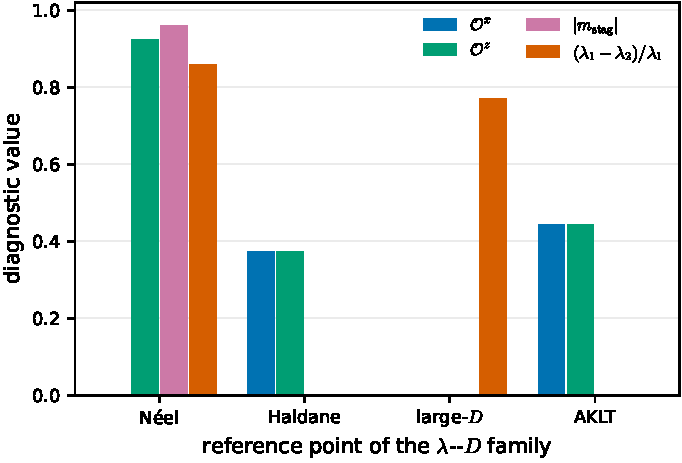
\includegraphics[width=0.78\textwidth]{figures/lambdaD-phase-points.pdf}
\caption{Ground-state diagnostics of the spin-1 $\lambda$--$D$ chain
\cref{eq:num-lambdaD} at its four reference points, at the largest bond
dimension computed ($\chi=48$). The N\'eel point ($\Delta=2.5$, $D=0$) has
$\mathcal{O}^x = 10^{-23}$ but $\mathcal{O}^z = 0.9255$ and staggered
magnetisation $0.9603$; the Haldane point ($\Delta=1$, $D=0$) has
$\mathcal{O}^x = \mathcal{O}^z = 0.3743$ and an entanglement doublet that is
exactly degenerate at the resolution of the calculation; the large-$D$ point
($\Delta=1$, $D=2.5$) has both string orders zero and a split spectrum; the
AKLT point ($\Delta=1$, $D=0$, $K=\tfrac13$) reproduces its closed forms
$\mathcal{O}^x=\mathcal{O}^z=4/9$, $e=-2/3$ and $S=\log 2$ to the printed
digits. The figure makes the operational point of the whole programme:
$\mathcal{O}^z$ is \emph{large} in the N\'eel phase and therefore does not
distinguish it from Haldane, whereas $\mathcal{O}^x$ does.}
\label{fig:lambdaD-phase-points}
\end{figure}

\begin{figure}[t]
\centering
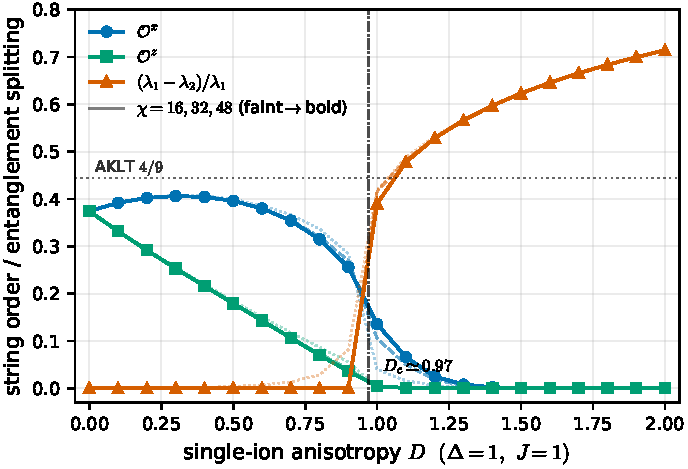
\includegraphics[width=0.78\textwidth]{figures/lambdaD-D-sweep.pdf}
\caption{The Haldane-to-large-$D$ sweep at $\Delta=1$: string order
parameters and the relative splitting of the leading entanglement doublet,
each recorded at $\chi=16,32,48$ (faint to bold) so that the bond-dimension
drift is visible. This is the rigidity dichotomy in one panel. The bulk
coefficient $\mathcal{O}^x$ \emph{drifts continuously} from its Heisenberg
value $0.374$ down through $0.256$ as $D$ approaches the transition, while the
entanglement doublet stays degenerate to below $5\times10^{-12}$ over the
whole Haldane side and then jumps by an $O(1)$ amount --- from
$4\times10^{-12}$ at $D=0.9$ to $0.39$ at $D=1.0$, eleven orders of magnitude
in one step of the sweep --- bracketing the literature value
$D_c\simeq0.97$. A quantised discrete datum survives exactly where a
continuous one is already sliding.}
\label{fig:lambdaD-D-sweep}
\end{figure}

\begin{figure}[t]
\centering
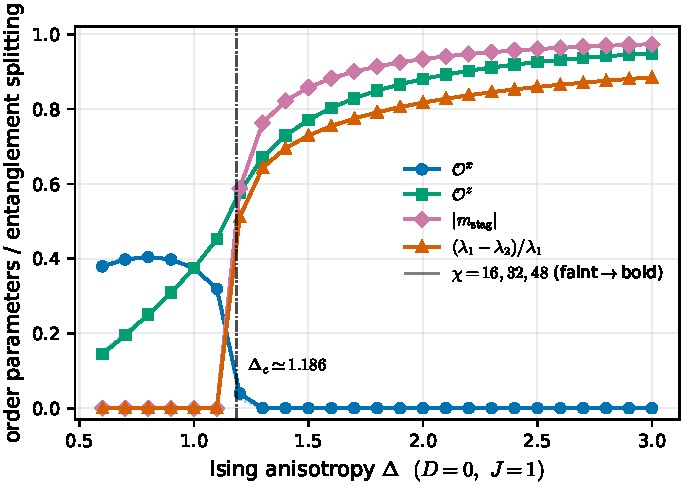
\includegraphics[width=0.78\textwidth]{figures/lambdaD-delta-sweep.pdf}
\caption{The Haldane-to-N\'eel sweep at $D=0$, on a two-site unit cell so that
the symmetry-broken state is representable. The staggered magnetisation and
the entanglement splitting switch on together between $\Delta=1.1$ (both below
$10^{-13}$) and $\Delta=1.2$ ($0.587$ and $0.511$ respectively), bracketing the
literature value $\Delta_c\simeq1.186$. $\mathcal{O}^x$ collapses across the
same window ($0.319 \to 0.039 \to 1.5\times10^{-4}$ at
$\Delta=1.1,1.2,1.3$), whereas $\mathcal{O}^z$ \emph{grows} straight through
the transition ($0.452 \to 0.577 \to 0.671$) and is therefore useless as a
phase discriminator here --- the point already made statically in
\cref{fig:lambdaD-phase-points}.}
\label{fig:lambdaD-delta-sweep}
\end{figure}

\Cref{fig:lambdaD-phase-points} fixes the four reference points and their
calibration. \Cref{fig:lambdaD-D-sweep,fig:lambdaD-delta-sweep} follow the
diagnostics across the two transitions. The headline is the one recorded in
\cref{sec:spt}: across the Haldane boundary the entanglement doublet is exact
until it is not, jumping by an $O(1)$ amount at a transition that a continuous
bulk order parameter merely drifts through. The critical points bracketed by
the jumps agree with the literature values $D_c\simeq0.97$ and
$\Delta_c\simeq1.186$.

Three controls support the reading. The AKLT point is a zero-parameter test of
nine closed-form numbers at once --- energy density, correlation length,
entropy, both string orders, exactly two Schmidt values each $1/\sqrt2$, a
vanishing doublet splitting, vanishing staggered order, and the exact
correlator $\langle S^z_1S^z_{1+r}\rangle = \tfrac43(-\tfrac13)^r$ out to
$r=8$ --- and it passes to the printed digits; in the charge-graded backend
the two Schmidt states are additionally found to sit in $S^z$ sectors exactly
one unit apart, which is the edge doublet read straight off the charge labels.
The Haldane doublet splitting reaches $9\times10^{-14}$ at the largest bond
dimension and stays below $5\times10^{-12}$ across the entire Haldane side of
the sweep, so the degeneracy is exact at the resolution of the calculation
rather than merely small. And the N\'eel point is deliberately run once more on
a \emph{one-site} unit cell, which cannot represent a symmetry-broken state and
is expected \emph{not} to converge: that failure is itself the evidence that
the breaking is physical, and the row is kept in the record with its
diagnostics visibly nonsensical.

Two caveats belong with these figures. The bond dimensions available on the
hardware used, $\chi\in\{16,32,48\}$, are not enough to resolve a critical
point: near a transition the correlation length and the string order are
$\chi$-limited, which is why every point is recorded at all three bond
dimensions rather than at the best one. And the reported correlation length is
the maximum over \emph{all} transfer-matrix channels, which need not be the
longitudinal channel that a $\langle S^zS^z\rangle$ fit sees; in the large-$D$
phase the two differ by more than a factor of two because the longest channel
there is transverse.

\provenance{--- (calibration and phase data for \cref{sec:spt})}
{--- (numerical record, no theorem asserted)}
{\texttt{numerics/\allowbreak{}results/\allowbreak{}lambdaD-\allowbreak{}phase-\allowbreak{}points.json} (17 rows),
 \texttt{lambdaD-\allowbreak{}D-\allowbreak{}sweep.json} (63 rows),
 \texttt{lambdaD-\allowbreak{}delta-\allowbreak{}sweep.json} (75 rows); produced by
 \texttt{numerics/\allowbreak{}scripts/\allowbreak{}run\_\allowbreak{}lambdaD\_\allowbreak{}phases.jl}; gated by
 \texttt{numerics/\allowbreak{}test/\allowbreak{}test\_\allowbreak{}lambdaD\_\allowbreak{}groundstate.jl}}
{bd lane \texttt{tns-f5r} wave 1}

\subsection{The \texorpdfstring{$\lambda$--$D$}{lambda-D} kink: dispersion and memory coefficient}\label{sec:numerics-kink}

The second production programme puts a kink of the N\'eel phase in motion and
measures what a magnon-like wavepacket does to it, in the non-integrable
setting of \cref{eq:num-lambdaD}. It runs at $\Delta=2.5$, $D=0$, $J=1$, deep
in the N\'eel phase, where the measured staggered tail density is
\begin{equation}
  s \;=\; m_{\text{stag}} \;=\; 0.960340 ,
  \label{eq:num-s}
\end{equation}
an ordinary number rather than a half-integer. This matters for reading the
prediction: the memory law of \cref{sec:memory-quantization} predicts the
coefficient $2s$, and $2s = 1.920680$ here.

\begin{figure}[t]
\centering
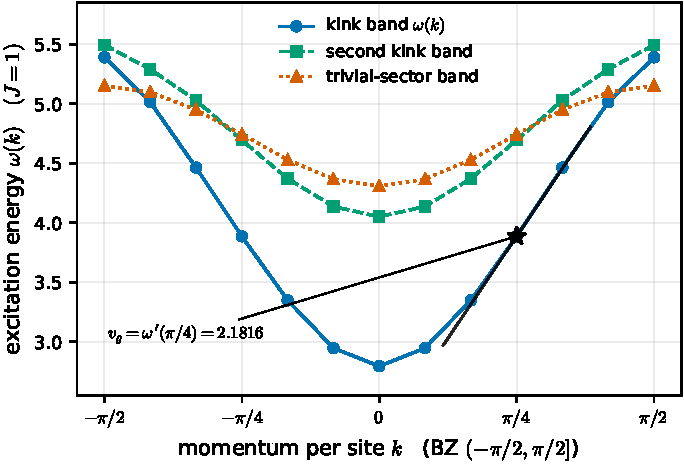
\includegraphics[width=0.78\textwidth]{figures/lambdaD-kink-dispersion.pdf}
\caption{Kink dispersion in the topological sector of the $\lambda$--$D$ chain
at $\Delta=2.5$, $D=0$, obtained from a quasiparticle excitation ansatz with
the two broken N\'eel vacua as left and right boundary conditions. Momentum is
per site, so $\omega(k)=\omega(k+\pi)$ and the zone is $(-\pi/2,\pi/2]$. The
kink band is gapped ($\Delta E = 2.7947$) with bandwidth $2.5957$ and is
cleanly separated from the second kink band and from the trivial-sector band
over the whole zone --- the separation that makes a single-band wavepacket
meaningful. The straight line is the tangent at the working momentum
$k_0=\pi/4$, giving $\omega(k_0)=3.886051$ and the group velocity
$v_g=2.181628$ against which the transport runs are calibrated. Three bond
dimensions ($\chi=16,24,32$) agree to nine significant figures, so only the
largest is drawn.}
\label{fig:lambdaD-kink-dispersion}
\end{figure}

\begin{figure}[t]
\centering
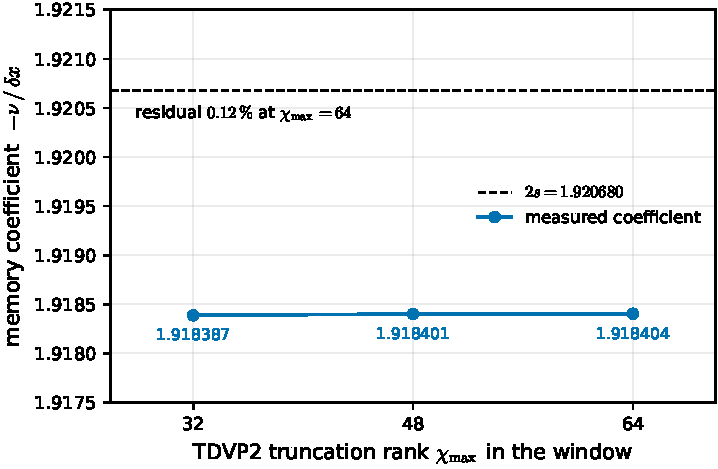
\includegraphics[width=0.78\textwidth]{figures/lambdaD-kink-memory-convergence.pdf}
\caption{Truncation-rank convergence of the measured memory coefficient
$-\delta x/\nu$ for the $\lambda$--$D$ kink transport at $L=48$, against the
predicted $2s=1.920680$ of \cref{eq:num-s}. Raising the two-site truncation
rank inside the evolution window from $\chi_{\max}=32$ to $64$ moves the
coefficient by $3.1\times10^{-6}$, from $1.9183874$ to $1.9184040$: the number
is converged in the truncation. The residual gap to $2s$ is $0.12$ per cent
and is a property of the finite window and readout geometry, not of the
truncation. The supporting quality gates are a norm drift of
$1.4\times10^{-6}$ and an energy drift of $2.6\times10^{-4}$ over the readout
interval.}
\label{fig:lambdaD-kink-memory-convergence}
\end{figure}

Two points about \cref{fig:lambdaD-kink-dispersion} matter for how the
transport numbers should be read. The band is \emph{computed}, not fitted: it
comes from a variational quasiparticle solve at each momentum, and the group
velocity is a central difference over three such solves. It is therefore fixed
\emph{before} any dynamics, and the measured wavepacket velocity is tested
against it rather than fitted to it. The wavepacket itself is built from the
variationally optimised excitation tensor at the working momentum; an
undressed step from one vacuum to the other is kept only as a deliberately bad
control, and it is bad by a wide margin --- its energy exceeds the band by
$9.8$, against a gate of $1.0$, where the dressed packet sits within
$3.7\times10^{-3}$ of $\omega(k_0)$.

\Cref{fig:lambdaD-kink-memory-convergence} then establishes that the memory
coefficient extracted from the transport is converged in the one parameter
that could plausibly have been controlling it. At the largest rank the run
measures a mean escaped charge $\nu=-16.372936$ and, with the $s$-free
centroid estimator, a wall displacement of $\delta x = 8.534665$ sites, giving
\begin{equation}
  -\frac{\nu}{\delta x} \;=\; 1.918404
  \qquad\text{against}\qquad 2s = 1.920680 ,
  \label{eq:num-coefficient}
\end{equation}
a deviation of $0.12$ per cent. Because the estimator on the left does not
contain $s$, this is a measurement of the coefficient and not an identity. The
measured propagation velocity in the window, $2.1343$, sits $2.2$ per cent
below the band value $2.1816$ of \cref{fig:lambdaD-kink-dispersion}, which is
the size one expects from a packet of finite width sampling the band
curvature.

The integer structure behind the law is certified separately, on the same
state and the same window. The windowed charge has
$|\langle e^{2\pi i\Qhat_W}\rangle| = 0.99995$ with a phase defect of
$5\times10^{-15}$ --- its spectrum lies in one coset of $\mathbb{Z}$, so every
escaped-charge outcome is an integer --- while the wall coordinate has
$|\langle e^{2\pi i\wallX_W}\rangle| = 0.438$, comfortably below one, as
it must be since $2s\notin\mathbb{Z}$. Displacing the window charge law's
weight to $1/(2s)$ turns the inversion into an aliased signed measure with
genuinely negative entries, and the test asserts that it does. The wall
displacement is not quantised; the charge is.

This is evidence for the memory law of \cref{sec:memory-quantization} in a
model with no integrability to lean on, and it is not a proof of anything. Two
limitations are stated in the source and should be stated here. First, the
protocol measures the \emph{bookkeeping} half of the memory statement: nothing
scatters off the wall in this run, so the displacement is ballistic transport
of a single packet, and a memory in the sense of a transient perturbation
leaving a permanent offset would require a second excitation inside the window
and is not attempted. Second, what is recorded is the exact single-time law of
the windowed charge at each sample; that coincides with the ordered two-point
measurement law of the theory only under the additional hypothesis named
there, which is carried in the record as an assumption and not as a result.

\provenance{--- (evidence for the memory law of \cref{sec:memory-quantization};
 no claim promoted)}
{--- (numerical record)}
{\texttt{numerics/\allowbreak{}results/\allowbreak{}lambdaD-\allowbreak{}kink-\allowbreak{}dispersion.json} (3 rows),
 \texttt{lambdaD-\allowbreak{}kink-\allowbreak{}memory-\allowbreak{}convergence.json} (3 rows); produced by
 \texttt{numerics/\allowbreak{}scripts/\allowbreak{}run\_\allowbreak{}lambdaD\_\allowbreak{}memory.jl}; gated by
 \texttt{numerics/\allowbreak{}test/\allowbreak{}test\_\allowbreak{}lambdaD\_\allowbreak{}memory.jl}}
{bd lane \texttt{tns-f5r} wave 2;
 \texttt{theory/\allowbreak{}lanes/\allowbreak{}blitz-\allowbreak{}2026-\allowbreak{}08-\allowbreak{}29/\allowbreak{}wave2-\allowbreak{}repair/\allowbreak{}SUMMARY.md}}

\subsection{The \texorpdfstring{$\lambda$--$D$}{lambda-D} edge: the memory contrast between phases}\label{sec:numerics-edge}

The third $\lambda$--$D$ experiment is the static counterpart of the
transport run. A ground state is prepared with boundary fields
$h_L=+\tfrac12$ and $h_R=-\tfrac12$ on a chain of $L=40$ sites, the left field
is switched off at $t=0$, and the magnetisation of the left half is followed.
The Haldane phase has a protected edge spin-$\tfrac12$ and should hold its
polarisation; the large-$D$ phase has no edge mode and should not acquire one.

\begin{figure}[t]
\centering
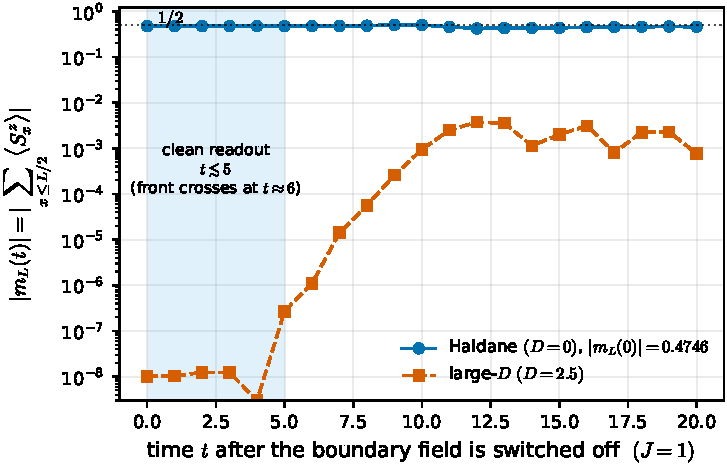
\includegraphics[width=0.78\textwidth]{figures/lambdaD-edge-memory.pdf}
\caption{Edge memory after the left boundary field is switched off, on a
logarithmic scale, for the Haldane point ($D=0$) and the trivial large-$D$
point ($D=2.5$) of the same Hamiltonian family, at $L=40$. The Haldane chain
carries $|m_L(0)| = 0.4746$, close to the half unit expected of a protected
edge spin-$\tfrac12$, and holds it; the large-$D$ chain never exceeds
$3.7\times10^{-3}$, a contrast of a factor $127$. The shaded band is the only
honest readout window: a bulk magnon front of speed $v\approx2.5$ reaches the
window edge at $t\approx6$, after which $|m_L|$ overshoots $\tfrac12$ because
bulk charge is crossing the window, not because the edge is decaying. Data
outside the band, including the record's $t=20$ "retention" field, is
front-contaminated (see \cref{sec:numerics-honesty}).}
\label{fig:lambdaD-edge-memory}
\end{figure}

\begin{figure}[t]
\centering
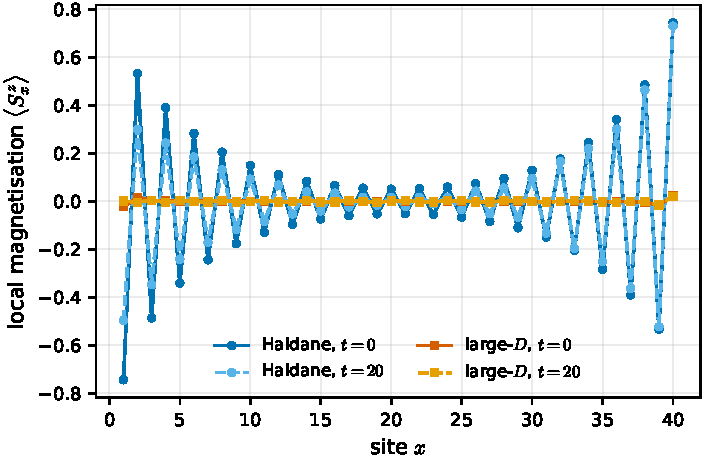
\includegraphics[width=0.78\textwidth]{figures/lambdaD-edge-profile.pdf}
\caption{Local magnetisation profiles for the same two runs, at preparation
and at the end of the evolution. The Haldane profile shows the staggered,
exponentially decaying edge moment characteristic of a fractionalised
boundary spin, essentially unchanged by the evolution; the large-$D$ profile
is flat at the resolution of the plot in both phases of the protocol. The
right-hand rise in the Haldane curves is the \emph{other} edge, which is
pinned by a permanent field for the whole run.}
\label{fig:lambdaD-edge-profile}
\end{figure}

\Cref{fig:lambdaD-edge-memory,fig:lambdaD-edge-profile} show the contrast.
Read together with \cref{eq:num-edge-fss}, which extrapolates the edge moment
to $\tfrac12$ as $L\to\infty$ with a decay length matching the spin-1
Heisenberg correlation length, they are the numerical face of the rigidity
statement of \cref{sec:spt}: a discrete, quantised boundary datum that a
trivial phase simply does not have.

Four caveats travel with these runs and are recorded in the data file. The
finite-chain Haldane retention is exact only up to the edge--edge splitting
time, which grows like $e^{L/\xi}$. The right edge is pinned throughout. The
choice $h_R=-h_L$ places both phases in the total-$S^z$ zero sector, so that
$m_L$ is a genuine measurement rather than half of a conserved total --- with
$h_R=+h_L$ the diagnostic would have been a symmetry artefact. And the
\emph{relative} retention of the large-$D$ run is a ratio of numerical zeros
and is meaningless; the absolute numbers are the ones to quote.

\provenance{--- (evidence for the boundary rigidity of \cref{sec:spt})}
{--- (numerical record)}
{\texttt{numerics/\allowbreak{}results/\allowbreak{}lambdaD-\allowbreak{}edge-\allowbreak{}memory.json} (2 rows); produced by
 \texttt{numerics/\allowbreak{}scripts/\allowbreak{}run\_\allowbreak{}lambdaD\_\allowbreak{}memory.jl}; gated by
 \texttt{numerics/\allowbreak{}test/\allowbreak{}test\_\allowbreak{}lambdaD\_\allowbreak{}memory.jl}}
{bd lane \texttt{tns-f5r} wave 2; open defect \texttt{tns-nkf}}

\subsection{The spin-\texorpdfstring{$s$}{s} falsifier battery}\label{sec:numerics-bc}

The conjecture at issue is the one discussed in \cref{sec:triangle-status}:
that the soft phase slope and the memory quantum are the same asymptotic
charge datum $|q_{\text{hard}}|/s$. At $s=\tfrac12$ both are $2$, which is
exactly the sort of coincidence that deserves to be attacked. The falsifier
was stated in advance: if the spin-1 phase slope is not $1$, the coincidence
is numerology and the conjecture must be dropped.

The analytic input is a contact solution of the spin-$S$ two-magnon problem,
obtained without any integrability assumption by keeping the free extension
$\Psi$ \emph{unsymmetrised} and matching on the physical chamber. Writing
$K=k_1+k_2$, $q=(k_1-k_2)/2$, $c=\cos(K/2)$ and
\begin{equation}
  n \;:=\; 2Sc\cos q - e^{iq}\bigl[(2S-1)c + \cos q\bigr],
  \label{eq:num-contact}
\end{equation}
the ratio is $S_{12} = n/(-\bar n)$, manifestly of unit modulus, and the soft
expansion gives
\begin{equation}
  \frac{\partial\delta}{\partial k_s}\Big|_{k_s=0} \;=\; \frac{1}{S},
  \label{eq:num-slope}
\end{equation}
with all hard-momentum dependence cancelling. At $S=\tfrac12$ the $(2S-1)c$
term vanishes and the expression collapses to the frozen $s=\tfrac12$ oracle
formula, checked to $10^{-12}$.

\begin{figure}[t]
\centering
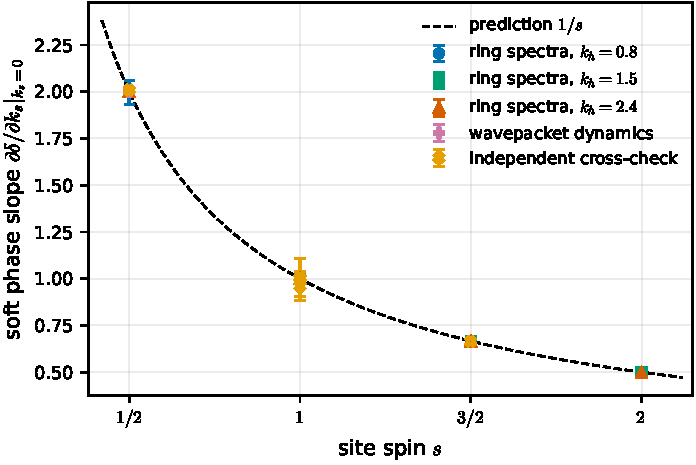
\includegraphics[width=0.78\textwidth]{figures/bc-soft-slope.pdf}
\caption{Measured soft phase slope $\partial\delta/\partial k_s|_0$ against
site spin, versus the predicted $1/s$. The ring points are \emph{ansatz-free}:
exact total-momentum-block spectra of the two-magnon sector are inverted
through $E=\omega(k_1)+\omega(k_2)$ and the Bethe--Yang quantisation
$Nk_s = 2\pi n_s + \delta$, extrapolated over
$N\in\{60,90,120,180,240,360,480\}$; no wavefunction ansatz and no $S$-matrix
enters. Independent wavepacket dynamics and an independent cross-check by
different methods are overlaid. Every one of the twelve ring determinations
lies within $0.003$ of $1/s$: $1.9979$--$2.0010$ at $s=\tfrac12$,
$0.9972$--$0.9995$ at $s=1$, $0.6645$--$0.6654$ at $s=\tfrac32$, and
$0.4978$--$0.4989$ at $s=2$. The prediction $2$ for every spin --- the outcome
that would have killed the conjecture --- is excluded by many standard
deviations at $s\geq1$.}
\label{fig:bc-soft-slope}
\end{figure}

\begin{figure}[t]
\centering
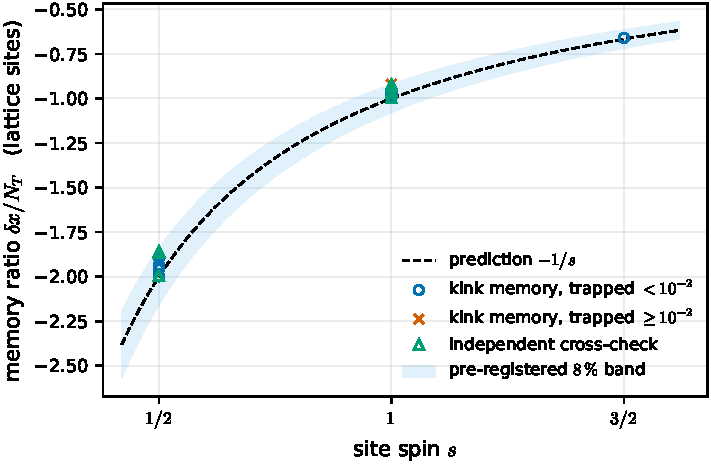
\includegraphics[width=0.78\textwidth]{figures/bc-memory-ratio.pdf}
\caption{The memory half of the same battery: measured ratio
$\delta x/N_T$ from spin-$s$ kink-transport runs, against the predicted
$-1/s$ and the pre-registered eight-per-cent decision band fixed before the
first run. Circles are runs whose trapped weight is below $10^{-2}$, so that
the asymptotic condition behind the law is actually met; crosses are the runs
where it is not. The nine spin-1 grid points average $-0.97996$, and the eight
of them with small trapped weight average $-0.98755$, within $1.3$ per cent of
$-1$; four spin-$\tfrac12$ controls on the same code path average $-1.97817$;
the single spin-$\tfrac32$ point gives $-0.66015$ against $-0.66667$ and is
the sharpest of all because it has only partial transmission ($T=0.383$), so
the ratio is not near-saturated.}
\label{fig:bc-memory-ratio}
\end{figure}

\Cref{fig:bc-soft-slope,fig:bc-memory-ratio} show both halves. Three
independent routes agree on the slope --- an exact-eigenvector residual test
at Bethe--Yang momenta, the ansatz-free ring extraction, and wavepacket
dynamics --- and across all $84$ ring rows the extracted phase agrees with the
analytic spin-$S$ expression to $8\times10^{-13}$. The memory ratio is
supported by size convergence (three chain lengths agreeing to five decimals),
by sharp-versus-dressed initial walls agreeing to $0.5$ per cent, and by the
basis-enlargement check quoted in \cref{sec:numerics-code}.

Two pieces of restraint belong with these numbers. The independent cross-check
records four of its fourteen memory runs as \emph{inconclusive} --- all at the
lower working momentum, where the packet is too broad in momentum for the
asymptotic reading and the two linear estimators bracket the prediction with a
spread of $0.17$ --- and those runs are kept in the published record with the
diagnosis attached rather than dropped. And the largest spin was reached only
at a reduced chain length: the corresponding sector needs of order twenty-four
gigabytes at the production size, and an attempt there was killed by the
operating system, so the $s=\tfrac32$ point is a single run on a shorter chain
and is the weakest of the battery.

The verdict is that the conjecture \emph{survived} both falsifiers. It remains
\statusConjecture. What the runs test sharply is the $1/s$ factor, since $s$
is varied over $\{\tfrac12,1,\tfrac32,2\}$; what they did not test is the
$|q_{\text{hard}}|$ factor, because every leg in every run carries unit
charge. That gap was later attacked directly: a three-magnon exact
diagonalisation at $N=100$ and $s=\tfrac12$, in which the hard leg is a
charge-two bound state, measured a slope of
\begin{equation}
  4.070 \pm 0.090 \qquad\text{against}\qquad |q_{\text{hard}}|/s = 4 ,
  \label{eq:num-charge2}
\end{equation}
inside a pre-registered absolute window of $0.35$, with a dense-sector oracle
running green and a deliberate mutation of the hopping running red. This too
is finite-packet evidence at a single volume and a single packet width: there
is no size or width extrapolation, and no charge-two kink-memory experiment
exists. The conjecture stays where it was.

\provenance{Bc}
{--- (conjecture; the slope half at unit charge is a separate proved row, see
 \cref{sec:two-magnon})}
{\texttt{numerics/\allowbreak{}results/\allowbreak{}spin1-\allowbreak{}bc-\allowbreak{}falsifier.json} ($84$ ring, $16$ dynamical,
 $22$ memory rows); \texttt{spin1-\allowbreak{}bc-\allowbreak{}crosscheck.json};
 \texttt{numerics/\allowbreak{}scripts/\allowbreak{}run\_\allowbreak{}spin1\_\allowbreak{}bc\_\allowbreak{}falsifier.jl},
 \texttt{run\_\allowbreak{}spin1\_\allowbreak{}bc\_\allowbreak{}crosscheck.jl}; decision tests in
 \texttt{numerics/\allowbreak{}test/\allowbreak{}test\_\allowbreak{}spins\_\allowbreak{}twomagnon.jl},
 \texttt{test\_\allowbreak{}spins\_\allowbreak{}memory.jl}, \texttt{test\_\allowbreak{}spin1\_\allowbreak{}twomagnon.jl},
 \texttt{test\_\allowbreak{}spin1\_\allowbreak{}memory.jl}}
{bd lane \texttt{tns-8e9}; charge-two lane
 \texttt{theory/\allowbreak{}lanes/\allowbreak{}blitz-\allowbreak{}2026-\allowbreak{}08-\allowbreak{}29/\allowbreak{}bc-\allowbreak{}charge2/\allowbreak{}}}

\subsection{The ferromagnetic two-magnon displacement scan}\label{sec:numerics-fm}

The soft theorem of \cref{sec:two-magnon} is derived algebraically. The
displacement scan tests it dynamically, and the test is genuinely independent:
the code never writes down a Bethe wavefunction. It enumerates down-spin
pairs, assembles the two-magnon Hamiltonian from the model directly, launches
two Gaussian packets in the incoming configuration --- hard behind soft, so
that the hard magnon overtakes --- and measures how far each outgoing packet
has been displaced relative to free propagation. By \cref{eq:num-wigner} those
displacements \emph{are} the momentum derivatives of the scattering phase, so
a sign error, a wrong branch or a swapped channel convention would show up
immediately.

\begin{figure}[t]
\centering
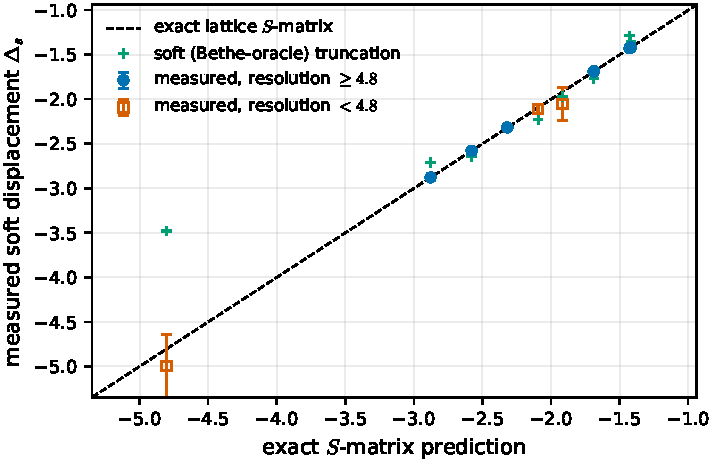
\includegraphics[width=0.78\textwidth]{figures/fm-displacement-soft.pdf}
\caption{Measured soft-magnon displacement $\Delta_s$ against the exact
lattice $S$-matrix prediction, for ten kinematic points of the spin-$\tfrac12$
isotropic Heisenberg ferromagnet; the dashed line is equality. Each point is
Richardson-extrapolated in $1/\sigma_x^2$ from packet widths
$\sigma_x\in\{8,11,14\}$, with the error bar the spread over all width pairs.
Every point agrees with the exact $S$-matrix inside its own error bar; where
the wavepacket geometry is well resolved the deviation is $3\times10^{-6}$ to
$5\times10^{-4}$, i.e.\ four to six significant digits of a scattering-phase
derivative recovered from real-time dynamics alone. The crosses are the soft
truncation of the theorem, which deviates visibly and by design --- most
dramatically at the leftmost point, where the soft hierarchy is deliberately
violated and the dynamics side with the exact $S$-matrix, confirming the
theorem's stated validity domain rather than refuting it.}
\label{fig:fm-displacement-soft}
\end{figure}

\begin{figure}[t]
\centering
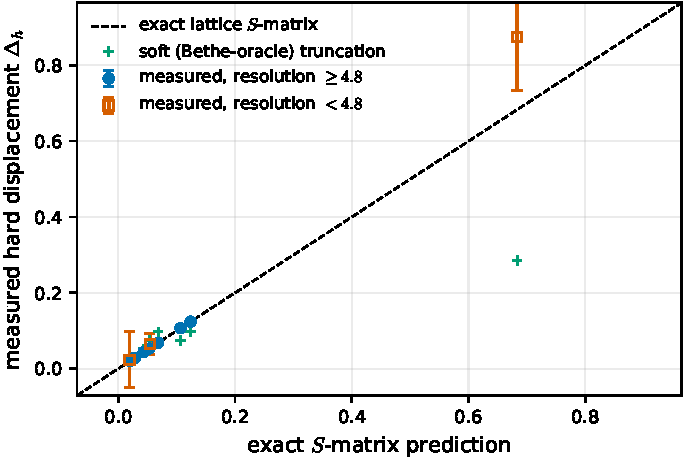
\includegraphics[width=0.78\textwidth]{figures/fm-displacement-hard.pdf}
\caption{The same comparison for the hard-magnon displacement $\Delta_h$.
It is positive in all ten runs and one to two orders of magnitude smaller than
$\Delta_s$ --- the classical hard-sphere pattern, with the overtaken particle
recoiling backwards by the contact length and the overtaking one jumping
forwards. This is the structural content of the soft theorem made visible: the
leading term of the phase carries no hard-momentum dependence and therefore
cannot displace the hard packet at all, so $\Delta_h$ is quadratic in the soft
momentum.}
\label{fig:fm-displacement-hard}
\end{figure}

\Cref{fig:fm-displacement-soft,fig:fm-displacement-hard} show the two
displacements. Beyond the pointwise agreement, the coefficients of the soft
expansion can be read off the dynamics with no $S$-matrix input at all, by
combining runs at $+k_s$ and $-k_s$: the antisymmetric combination isolates
the first hard invariant and the symmetric one the leading scattering length.
Extrapolating the two available soft momenta at fixed hard momentum gives
$2.147178$ for the former, against $2.147197$ from the exact lattice
$S$-matrix and $2\cot(k_h/2) = 2.146852$ from the theorem, and the latter
converges to $2$ within $0.2$ per cent. \textbf{The leading, hard-data
independent scattering length $2$ is a directly measured lattice
displacement}, not an artefact of an ansatz.

The one place where the dynamical method is strictly weaker than the algebra
is kinematic rather than analytic: as the hard momentum approaches $\pi$ its
group velocity vanishes, the incoming condition becomes almost unsatisfiable,
and the collision takes $O(10^3)$ time units. The accuracy is controlled by a
single dimensionless resolution --- final separation over combined final
packet width --- and, because dispersive spreading grows with the propagation
time, pushing the packets further apart does not improve it; only fatter
packets or a faster relative velocity do, at cost cubic in the packet width.

The related claim row \texttt{N1}, that excitation-ansatz magnon amplitudes
reproduce the Bethe $S$-matrix in the soft limit, has \emph{not} been run and
remains \statusConjecture\ with no supporting data.

\provenance{N1 (not run); supporting data for the two-magnon soft expansion of
 \cref{sec:two-magnon}}
{--- (numerical record)}
{\texttt{numerics/\allowbreak{}results/\allowbreak{}fm-\allowbreak{}displacement-\allowbreak{}scan.json} ($10$ summary rows over
 $30$ evolutions); produced by \texttt{numerics/\allowbreak{}src/\allowbreak{}fm\_\allowbreak{}twomagnon.jl};
 gated by \texttt{numerics/\allowbreak{}test/\allowbreak{}test\_\allowbreak{}fm\_\allowbreak{}twomagnon.jl}}
{\texttt{numerics/\allowbreak{}docs/\allowbreak{}fm-\allowbreak{}twomagnon-\allowbreak{}notes.md}}

\subsection{The XXZ kink-memory scan}\label{sec:numerics-xxz}

The last family is the original spin-$\tfrac12$ memory experiment: a magnon
wavepacket sent at a kink in the easy-axis chain \cref{eq:num-xxz}, with the
displacement of the kink measured before and after.

The bookkeeping argument is worth stating because it is what the data
confirms. Before the collision the state is a kink at $X$ plus one extra down
spin in the up region. After full transmission the magnon is an \emph{up}
bubble in the down region, at the same total $S^z$. The wall must absorb the
difference, and it can only do so by moving two sites. Hence a transmitted
magnon displaces the kink by exactly $-2$ sites, a reflected one by zero, and
\begin{equation}
  \delta x \;=\; -2\,T ,
  \label{eq:num-dx2T}
\end{equation}
so the memory is quantised and the whole of its magnitude sits in the
transmission probability. On the lattice the collective coordinate can only
shift in units of two sites and the continuous observable is the \emph{weight}
$T$, not the displacement.

\begin{figure}[t]
\centering
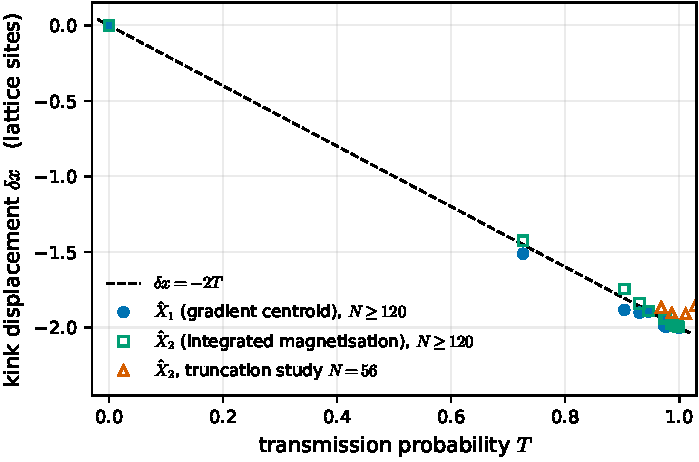
\includegraphics[width=0.78\textwidth]{figures/xxz-memory-dx-vs-T.pdf}
\caption{Kink displacement against transmission probability for the
spin-$\tfrac12$ XXZ memory scan, with the prediction $\delta x = -2T$ of
\cref{eq:num-dx2T} as the dashed line. Production runs at $N\geq120$ are shown
for both linear estimators; the $N=56$ points are the truncation study, whose
geometry carries much larger systematics. Over the whole scan
$|\delta x_1 + 2T| \leq 0.075$, and at the cleanest geometries --- those with
trapped weight below $10^{-6}$ --- the residual is $0.004$ sites. Three chain
lengths $N=120,160,200$ reproduce the same numbers to six significant figures,
and an Ising control with the exchange switched off returns
$T=0$, $R=1$ and $\delta x=0$ exactly.}
\label{fig:xxz-memory-dx-vs-T}
\end{figure}

\begin{figure}[t]
\centering
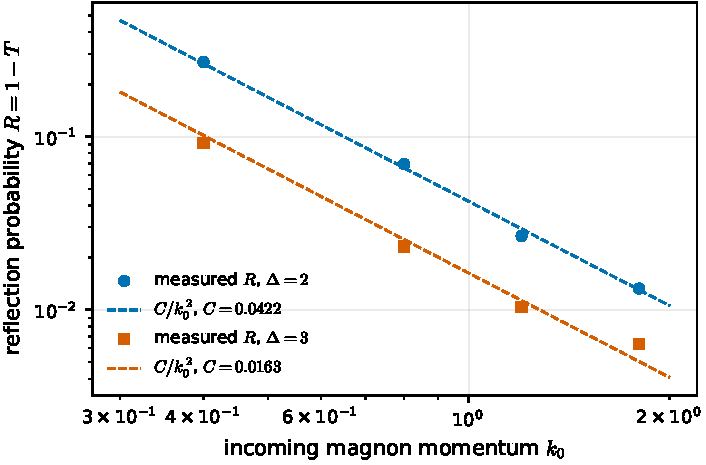
\includegraphics[width=0.78\textwidth]{figures/xxz-reflection-threshold.pdf}
\caption{Reflection probability against incoming magnon momentum, on
logarithmic axes, at two anisotropies, with fitted curves $C(\Delta)/k_0^2$.
The measured $R$ follows the one-dimensional low-energy threshold law with
$C(2)\approx0.042$ and $C(3)\approx0.016$, so $T\to0$ and, by
\cref{eq:num-dx2T}, $\delta x\to0$ as $k_0\to0$: \emph{a soft magnon leaves no
memory}. This is the model's Adler-type zero, and it is the qualitative
content of the soft theorem seen from the memory side. In the same regime
$C(\Delta)$ falls like $\Delta^{-2}$, so the kink becomes \emph{more}
transparent, and the memory closer to its quantum, the deeper the easy axis.}
\label{fig:xxz-reflection-threshold}
\end{figure}

\Cref{fig:xxz-memory-dx-vs-T} is the quantitative statement and
\cref{fig:xxz-reflection-threshold} the physical one. A refuted prior
expectation belongs here too, since it was recorded before the runs: it was
predicted that at large anisotropy the kink would be an opaque barrier. It is
not. Transmission tends to \emph{one} as $\Delta\to\infty$. The mechanism is
visible in the domain-wall algebra --- the elementary exchange move takes a
magnon adjacent to the wall on the up side directly into a bubble on the down
side, displacing the wall by two, so transmission is a first-order,
energy-conserving process inside the retained manifold, while the merge
channel that produces reflection is off-resonant by one magnon gap. The
easy-axis kink is nearly transparent to magnons, and the more so the deeper
the easy axis. This is the numerical face of the decoupling statement of
\cref{sec:kink-model}: the magnon couples to the wall's collective coordinate
and to nothing else.

This is the evidence behind claim row \texttt{N2}, and it is held at
\statusSketch. The row says exactly what it is: an empirical scan matching the
conditional memory expectation at the recorded precision, $\delta x \approx
-2T$ to within $0.004$ sites. It is numerical evidence, not a theorem, and it
does not promote the conditional theorem it agrees with.

\provenance{N2 \statusSketch}
{--- (empirical scan only; the theorem it agrees with is conditional and lives
 in \cref{sec:memory-quantization})}
{\texttt{numerics/\allowbreak{}results/\allowbreak{}memory-\allowbreak{}scan-\allowbreak{}1.json} ($21$ runs); produced by
 \texttt{numerics/\allowbreak{}scripts/\allowbreak{}run\_\allowbreak{}memory\_\allowbreak{}scan.jl} over
 \texttt{numerics/\allowbreak{}src/\allowbreak{}xxz\_\allowbreak{}sector.jl}, \texttt{xxz\_\allowbreak{}dynamics.jl},
 \texttt{memory\_\allowbreak{}experiment.jl}; gated by
 \texttt{numerics/\allowbreak{}test/\allowbreak{}test\_\allowbreak{}xxz\_\allowbreak{}sector.jl},
 \texttt{test\_\allowbreak{}xxz\_\allowbreak{}dynamics.jl}, \texttt{test\_\allowbreak{}memory\_\allowbreak{}experiment.jl}}
{\texttt{numerics/\allowbreak{}docs/\allowbreak{}kink-\allowbreak{}sector-\allowbreak{}notes.md}}

\subsection{Honesty: defects, quarantine, and what none of this proves}\label{sec:numerics-honesty}

\subsubsection*{A quarantined record}

The $\lambda$--$D$ transport production stage produced one record that is
\emph{not} a result and is not plotted anywhere in this section. The file
\texttt{numerics/\allowbreak{}results/\allowbreak{}lambdaD-\allowbreak{}kink-\allowbreak{}memory.FAILED-\allowbreak{}NaN.json} is quarantined
under a name that says so.

What happened is this. The stage ran two rows at $L=72$, one for each initial
dressing of the kink. The evolution itself was clean in both: energies, norms
and position time series are finite throughout, out to $t=14$. The first row,
with a quasiparticle-dressed initial kink, completed normally and reported a
coefficient of $1.9131$ against $2s=1.920680$. The second row, with a
deliberately undressed sharp kink, has \emph{every} analysis output
non-finite: measured velocity, all three displacement estimators, the mean
escaped charge and the coefficient.

The mechanism is visible in the record and is worth stating precisely, because
it is more specific than "the fit broke". The readout interval is selected by
requiring both that the wall be padded from the window edges and that the
measured edge leakage stay below a fixed tolerance of $10^{-3}$. For the sharp
preparation the leakage starts at $5\times10^{-3}$ --- already five times the
tolerance at $t=0$ --- and grows monotonically to $0.159$. No sample ever
qualifies, the recorded readout index range is empty, and the analysis
correctly declines to compute a displacement outside the region where its
definition applies, returning non-finite values instead. That branch is doing
what its specification promises, and for an undressed junction, which is not a
one-kink state at all, declining is arguably the right answer.

The defects are therefore not where one first looks. The first is that a
production stage \emph{wrote its output file and exited with status zero} while
producing nothing but non-finite numbers; this is the same species of failure
as a test gate that cannot fail, and it is why the record was committed
silently. The second is that there is no finiteness gate anywhere in the
driver. Both are tracked as an open priority-one defect (bd
\texttt{tns-kng}), along with the requirement to rerun. A third question is
open rather than defective: even the surviving row's readout interval was
closed by the end of the integration rather than by the physics, so whether
its numbers should be re-derived on a longer run is undecided.

Until this is resolved there is no \texttt{lambdaD-\allowbreak{}kink-\allowbreak{}memory.json}, and the
converged coefficient of \cref{fig:lambdaD-kink-memory-convergence} --- which
comes from a separate, regenerated convergence record at $L=48$, independently
recomputed from raw fields --- is the only transport number this labbook
quotes.

\subsubsection*{A mismeasured diagnostic}

The edge-memory record carries a field named \texttt{retention}, evaluated at
$t=20$, reading $0.971$ for the Haldane run. That number is
front-contaminated and should not be quoted. As \cref{fig:lambdaD-edge-memory}
shows, the left-half magnetisation is frozen to within $7\times10^{-6}$ for
$t\leq5$ and then a bulk magnon front crosses the window edge at $t\approx6$,
pushing $|m_L|$ past $\tfrac12$ --- bulk charge entering the window, not edge
memory persisting. The honest readout window is $t\lesssim L/2v$, and the
module docstring at present caveats only the far longer edge--edge splitting
time. The quantities to quote are the initial, final and extremal values of
$m_L$ within the clean window, and the contrast between the phases, which is
robust: a factor of $127$ in the edge moment. This is an open documentation
and record defect (bd \texttt{tns-nkf}).

\subsubsection*{Estimator hazards, recorded}

Three estimator lessons are worth carrying, all of them learned by a test
failing. A windowed centroid of the one-body density looks unimpeachable and
is biased at the ten-per-cent level by dispersively spread tails, and it
jumps discretely as an integer window edge moves --- it produced the wrong
\emph{sign} for the hard-magnon displacement, which would have appeared to
falsify a correct theorem. The zero-crossing wall estimator $\hat X_3$ is
quantised on mixtures and jumps as branch weights cross one half; it is a
diagnostic and must never be used interchangeably with the linear estimators
at partial transmission. And the transmission and reflection integrals of
\cref{eq:num-TR} are normalised only in the one-magnon sector: in an enlarged
basis, virtual magnon pairs contribute their own up and down density and
$T+R$ can exceed one, with the trapped weight going negative. Two runs in the
scans exhibit exactly that, and are labelled accordingly.

A fourth lesson was promoted from a bug into an invariant. An early spin-$s$
memory run returned a ratio of $-1.104$ where the raw before-and-after
difference of the wall position was $-1.02$. The cause was geometric: the
packet was not yet asymptotic at $t=0$, so it already overlapped the
reflected-weight region, the trapped weight never fell below tolerance, the
data-driven pre-collision window degenerated to a three-point geometric
fallback, and that window's spurious slope was extrapolated across the whole
interval. The fix was not a tolerance but a hard precondition, now enforced by
the code, that the standoff exceed the buffer by at least four packet widths
--- at which separation only $3\times10^{-5}$ of the packet lies outside, an
order of magnitude below the trapped tolerance. There is now a test asserting
that the protocol \emph{refuses} a non-asymptotic geometry, and the decision
band was left unchanged.

Two further reporting rules are baked into the records, and a reader should
know them. A quantity a given code path cannot represent is written as
not-a-number, never as zero --- so a zero in these files means a measurement,
not an absence. And a bond whose numerical rank falls short of its nominal
bond dimension is flagged, because the transfer spectrum then contains
null-space artefacts; the affected correlation length is nulled while the raw
value is retained for inspection, and there is a test asserting that the raw
value is finite \emph{and wrong}.

\subsubsection*{What is evidence and what is proof}

To be explicit, because this is the point on which a reader could most easily
be misled.

The numbers in \cref{sec:numerics-phases,sec:numerics-kink,sec:numerics-edge,%
sec:numerics-bc,sec:numerics-fm,sec:numerics-xxz} are \emph{evidence}. Some of
it is very strong: a scattering-phase derivative reproduced to six significant
figures from real-time dynamics, a memory coefficient converged in its
truncation to six decimals, twelve independent determinations of a slope all
within $0.003$ of a prediction that a competing hypothesis puts a factor of
two away. None of it is proof, and none of it changes a status.

Concretely: the conjecture attacked in \cref{sec:numerics-bc} survived its
falsifiers and remains \statusConjecture; the empirical scan of
\cref{sec:numerics-xxz} is \statusSketch\ and stays there; the row on
excitation-ansatz amplitudes is \statusConjecture\ and has no data at all. The
theorems these experiments accompany are proved, where they are proved,
elsewhere in this document and by the arguments recorded there --- and where
they are conditional, as in \cref{sec:memory-quantization}, agreement with a
numerical experiment does not discharge the condition.

\subsection{Provenance of every record}\label{sec:numerics-provenance}

For reference, each committed results file with the script that produced it
and the tests that gate it. All paths are relative to the repository root.

% Long path lists: relax the line breaker for this listing only.
\begingroup\sloppy

\texttt{numerics/\allowbreak{}results/\allowbreak{}fm-\allowbreak{}displacement-\allowbreak{}scan.json} --- produced by the
displacement-scan driver in \texttt{numerics/\allowbreak{}src/\allowbreak{}fm\_\allowbreak{}twomagnon.jl}; gated by
\texttt{numerics/\allowbreak{}test/\allowbreak{}test\_\allowbreak{}fm\_\allowbreak{}twomagnon.jl}; documented in
\texttt{numerics/\allowbreak{}docs/\allowbreak{}fm-\allowbreak{}twomagnon-\allowbreak{}notes.md}.

\texttt{numerics/\allowbreak{}results/\allowbreak{}memory-\allowbreak{}scan-\allowbreak{}1.json} --- produced by
\texttt{numerics/\allowbreak{}scripts/\allowbreak{}run\_\allowbreak{}memory\_\allowbreak{}scan.jl} over
\texttt{numerics/\allowbreak{}src/\allowbreak{}xxz\_\allowbreak{}sector.jl}, \texttt{xxz\_\allowbreak{}dynamics.jl} and
\texttt{memory\_\allowbreak{}experiment.jl}; gated by
\texttt{numerics/\allowbreak{}test/\allowbreak{}test\_\allowbreak{}xxz\_\allowbreak{}sector.jl},
\texttt{test\_\allowbreak{}xxz\_\allowbreak{}dynamics.jl} and \texttt{test\_\allowbreak{}memory\_\allowbreak{}experiment.jl};
documented in \texttt{numerics/\allowbreak{}docs/\allowbreak{}kink-\allowbreak{}sector-\allowbreak{}notes.md}.

\texttt{numerics/\allowbreak{}results/\allowbreak{}spin1-\allowbreak{}bc-\allowbreak{}falsifier.json} --- produced by
\texttt{numerics/\allowbreak{}scripts/\allowbreak{}run\_\allowbreak{}spin1\_\allowbreak{}bc\_\allowbreak{}falsifier.jl} over
\texttt{numerics/\allowbreak{}src/\allowbreak{}spin1\_\allowbreak{}twomagnon.jl}, \texttt{spin1\_\allowbreak{}collision.jl},
\texttt{spin1\_\allowbreak{}memory.jl}, \texttt{spin1\_\allowbreak{}memory\_\allowbreak{}run.jl},
\texttt{spins\_\allowbreak{}twomagnon.jl}, \texttt{spins\_\allowbreak{}twomagnon\_\allowbreak{}sector.jl},
\texttt{spins\_\allowbreak{}twomagnon\_\allowbreak{}collision.jl}, \texttt{spins\_\allowbreak{}memory.jl},
\texttt{spins\_\allowbreak{}memory\_\allowbreak{}sector.jl} and \texttt{spins\_\allowbreak{}memory\_\allowbreak{}run.jl}; gated by
\texttt{numerics/\allowbreak{}test/\allowbreak{}test\_\allowbreak{}spin1\_\allowbreak{}twomagnon.jl},
\texttt{test\_\allowbreak{}spin1\_\allowbreak{}memory.jl}, \texttt{test\_\allowbreak{}spins\_\allowbreak{}twomagnon.jl} and
\texttt{test\_\allowbreak{}spins\_\allowbreak{}memory.jl}; documented in
\texttt{numerics/\allowbreak{}docs/\allowbreak{}spin1-\allowbreak{}twomagnon-\allowbreak{}notes.md}.

\texttt{numerics/\allowbreak{}results/\allowbreak{}spin1-\allowbreak{}bc-\allowbreak{}crosscheck.json} --- produced by
\texttt{numerics/\allowbreak{}scripts/\allowbreak{}run\_\allowbreak{}spin1\_\allowbreak{}bc\_\allowbreak{}crosscheck.jl}, by deliberately
different methods from the file above; gated by the same test files.

\texttt{numerics/\allowbreak{}results/\allowbreak{}lambdaD-\allowbreak{}phase-\allowbreak{}points.json},
\texttt{lambdaD-\allowbreak{}D-\allowbreak{}sweep.json} and \texttt{lambdaD-\allowbreak{}delta-\allowbreak{}sweep.json} ---
produced by \texttt{numerics/\allowbreak{}scripts/\allowbreak{}run\_\allowbreak{}lambdaD\_\allowbreak{}phases.jl} over
\texttt{numerics/\allowbreak{}src/\allowbreak{}lambdaD\_\allowbreak{}model.jl} and
\texttt{lambdaD\_\allowbreak{}diagnostics.jl}; gated by
\texttt{numerics/\allowbreak{}test/\allowbreak{}test\_\allowbreak{}lambdaD\_\allowbreak{}groundstate.jl}.

\texttt{numerics/\allowbreak{}results/\allowbreak{}lambdaD-\allowbreak{}kink-\allowbreak{}dispersion.json},
\texttt{lambdaD-\allowbreak{}kink-\allowbreak{}memory-\allowbreak{}convergence.json} and
\texttt{lambdaD-\allowbreak{}edge-\allowbreak{}memory.json} --- produced by
\texttt{numerics/\allowbreak{}scripts/\allowbreak{}run\_\allowbreak{}lambdaD\_\allowbreak{}memory.jl} over
\texttt{numerics/\allowbreak{}src/\allowbreak{}lambdaD\_\allowbreak{}memory.jl},
\texttt{lambdaD\_\allowbreak{}memory\_\allowbreak{}run.jl} and \texttt{lambdaD\_\allowbreak{}edge.jl}; gated by
\texttt{numerics/\allowbreak{}test/\allowbreak{}test\_\allowbreak{}lambdaD\_\allowbreak{}memory.jl}.

\texttt{numerics/\allowbreak{}results/\allowbreak{}lambdaD-\allowbreak{}kink-\allowbreak{}memory.FAILED-\allowbreak{}NaN.json} ---
\textbf{quarantined}, produced by the same transport driver; not gated, not
plotted, and not to be cited as a result. See
\cref{sec:numerics-honesty} and bd \texttt{tns-kng}.

The figures of this section are regenerated from these records by
\texttt{labbook/\allowbreak{}figures/\allowbreak{}make\_\allowbreak{}figures.py}, which reads only the JSON files
listed above and writes the PDFs referenced in the figure environments. Any
rerun of the numerics must be followed by a rerun of that script, in the same
commit, under the lockstep rule.
\endgroup

\endgroup
